% ******************************************************** %
%              TEMPLATE DE INFORME ORGA2 v0.1              %
% ******************************************************** %
% ******************************************************** %
%                                                          %
% ALGUNOS PAQUETES REQUERIDOS (EN UBUNTU):                 %
% ========================================
%                                                          %
% texlive-latex-base                                       %
% texlive-latex-recommended                                %
% texlive-fonts-recommended                                %
% texlive-latex-extra?                                     %
% texlive-lang-spanish (en ubuntu 13.10)                   %
% ******************************************************** %


\documentclass[a4paper]{article}
\usepackage[spanish]{babel}
\usepackage[utf8]{inputenc}
\usepackage{charter}   % tipografia
\usepackage{graphicx}
%\usepackage{makeidx}
\usepackage{paralist} %itemize inline
\usepackage{float}

%\usepackage{float}
%\usepackage{amsmath, amsthm, amssymb}
%\usepackage{amsfonts}
%\usepackage{sectsty}
%\usepackage{charter}
%\usepackage{wrapfig}
%\usepackage{listings}
%\lstset{language=C}

% \setcounter{secnumdepth}{2}
\usepackage{underscore}
\usepackage{caratula}
\usepackage{url}


% ********************************************************* %
% ~~~~~~~~              Code snippets             ~~~~~~~~~ %
% ********************************************************* %

\usepackage{color} % para snipets de codigo coloreados
\usepackage{fancybox}  % para el sbox de los snipets de codigo

\definecolor{litegrey}{gray}{0.94}

\newenvironment{codesnippet}{%
	\begin{Sbox}\begin{minipage}{\textwidth}\sffamily\small}%
	{\end{minipage}\end{Sbox}%
		\begin{center}%
		\vspace{-0.4cm}\colorbox{litegrey}{\TheSbox}\end{center}\vspace{0.3cm}}



% ********************************************************* %
% ~~~~~~~~         Formato de las páginas         ~~~~~~~~~ %
% ********************************************************* %

\usepackage{fancyhdr}
\pagestyle{fancy}

%\renewcommand{\chaptermark}[1]{\markboth{#1}{}}
\renewcommand{\sectionmark}[1]{\markright{\thesection\ - #1}}

\fancyhf{}

\fancyhead[LO]{Sección \rightmark} % \thesection\ 
\fancyfoot[LO]{\small{Nombre Apellido, Nombre Apellido, Nombre Apellido}}
\fancyfoot[RO]{\thepage}
\renewcommand{\headrulewidth}{0.5pt}
\renewcommand{\footrulewidth}{0.5pt}
\setlength{\hoffset}{-0.8in}
\setlength{\textwidth}{16cm}
%\setlength{\hoffset}{-1.1cm}
%\setlength{\textwidth}{16cm}
\setlength{\headsep}{0.5cm}
\setlength{\textheight}{25cm}
\setlength{\voffset}{-0.7in}
\setlength{\headwidth}{\textwidth}
\setlength{\headheight}{13.1pt}

\renewcommand{\baselinestretch}{1.1}  % line spacing

% ******************************************************** %


\begin{document}


\thispagestyle{empty}
\materia{Organización del Computador II}
\submateria{Segundo Cuatrimestre de 2016}
\titulo{Trabajo Práctico II}
\subtitulo{Operaciones con SIMD}
\integrante{Nombre}{XXX/XX}{mail}
\integrante{Nombre}{XXX/XX}{mail}

\maketitle
\newpage

\thispagestyle{empty}
\vfill
\begin{abstract}
En este trabajo se presentan implementaciones sobre el procesamiento de imágenes de manera tal que se computen los datos de forma vectorizada, utilizando la tecnología SIMD de Intel para procesar varios de ellos simultáneamente y así obtener un mejor rendimiento. Luego se presentan distintas aproximaciones a los problemas, presentando hipótesis y experimentaciones en base a su rendimiento que permiten comprobarlas o refutarlas según un determinado criterio.
\end{abstract}

\thispagestyle{empty}
\vspace{3cm}
\tableofcontents
\newpage


%\normalsize
\newpage

\section{Objetivos generales}

El objetivo de este Trabajo Práctico es comprender el uso de las instrucciones que aprovechan la tecnología SIMD de Intel para procesar varios datos simultáneamente, en conjunto con un análisis con respecto a las implementaciones realizadas para lograr un mayor entendimiento de su funcionamiento y a su vez de cómo plantear y analizar distintas problemáticas sobre un mismo tema.


\section{Contexto}

%--------------Acá ponemos lo que aplica a todos los filtros-----------------

%\begin{figure}
%  \begin{center}
%	
\includegraphics[scale=0.66]{imagenes/logouba.jpg}
%	\caption{Descripcion de la figura}
%	\label{nombreparareferenciar}
%  \end{center}
%\end{figure}

Para la implementación y uso de las instrucciones SIMD, se trabaja sobre el procesamiento de imágenes, aplicando distintos filtros sobre los mismos. Las imágenes se almacenan en memoria como una matriz con elementos de 32 bits, donde cada elemento corresponde a un pixel de la imagen. Para las implementaciones sobre C, se utiliza la siguiente estructura provisto en \textit{tp2.h} para trabajar sobre los pixeles:
%\paragraph{\textbf{Titulo del parrafo} } Bla bla bla bla.
%Esto se muestra en la figura~\ref{nombreparareferenciar}.
\begin{codesnippet}
\begin{verbatim}

typedef struct bgra_t {
	unsigned char b, g, r, a;
} __attribute__((packed)) bgra_t;

\end{verbatim}
\end{codesnippet}

Además, para las mediciones de rendimiento, se cuentan la cantidad de \textit{ticks} del procesador que conllevó ejecutar una determinada implementación de los filtros. Los datos de entrada varían en igual cantidad en tamaño y ancho. No se analizan distintas imágenes porque sus componentes no interfieren en los cálculos realizados por los filtros; es decir, el rendimiento de los filtros es independiente de las componentes cromáticas de las imágenes (el único que trabaja en base a los valores de los colores es \textit{Colorizar}, el por qué no lo afectan se encuentra en la explicación de su implementación).

Los filtros se corren cien veces en total y se obtiene un promedio del mismo. La carga y guardado de imágenes se ejecuta anterior y posteriormente a la corrida del filtro, por lo que no afecta a las mediciones. Para evitar la presencia de \textit{outliers}, se calcula la desviación estándar de las mediciones. Si la misma es mayor o solo un 10\% menor al promedio, se descarta la medición y se realiza devuelta.

El código utilizado para las mediciones se encuentra en el archivo \textit{tp2.c}, método \textit{void correr_filtro_imagen}.
\newpage
\section{Filtros} 
\subsection{Smalltiles}
\subsubsection{Implementación}
Este filtro implica dividir la imagen original en cuatro cuadrantes, manteniendo el tamaño original. Para generar cada cuadrante, recorremos la imagen original salteando una fila y columna de por medio. Es decir, cuando procesamos un pixel, descartamos a su vecino y lo almacenamos en cada una de las posiciones de los cuadrantes en la imagen destino, las cuales las calculamos mediante la cantidad de columnas y filas de la imagen fuente (dividiendo por la mitad y multiplicando por el tamaño de los datos de la matriz (32 bits)). Luego, al terminar de recorrer la fila, salteamos la siguiente fila (sumándole al puntero de la imagen fuente el tamaño de la fila en bytes).

Debido a que solo recorremos la mitad de las filas, la cantidad de iteraciones que se realizan equivale a la cantidad de columnas multiplicado por la cantidad de filas dividido dos. Ya que se itera por columnas, en la implementación en lenguaje ensamblador se mantiene un contador que aumenta en cada iteración y, una vez que se alcanzó la cantidad total de columnas, se asume que se terminó de recorrer la fila y se realizan las operaciones pertinentes para mover los punteros a la fila posterior a la siguiente en memoria (se saltea una fila, como se explicó anteriormente).
\bigskip

El procesamiento en lenguaje ensamblador se realiza de a cuatro pixeles por iteración, por lo que se divide la cantidad total de columnas por cuatro. No es posible procesar de a más pixeles a la vez porque cada uno ocupa 4 bytes y solo entran cuatro de ellos en los registros de SIMD. Dado que el filtro consta básicamente de reordenar datos, se utiliza una única instrucción para su procesamiento. La misma es la instrucción \textit{shuffle}, la cual se ejecuta de manera tal que por cada cuatro pixeles en el registro, se ubican de forma subsiguiente a aquellos de la primera y tercera columna y se los almacena en memoria en cada puntero a cada cuadrante de la imagen destino, descartando a los otros dos.
\bigskip

Dentro de la implementación en C, se recorre la imagen fuente iterando una cantidad de veces equivalente a $\frac{filas}{2} * \frac{cols}{2}$, lo cual representa al tamaño de la imagen de cada cuadrante. De esta manera, el programa selecciona los pixeles de fila y columna par, los cuales son los que se guardarán en la imagen destino. Se itera píxel por píxel, donde en cada iteración se crean cuatro punteros a las direcciones de memoria correspondientes a cada cuadrante de la imagen destino.

Ya que se procesa una mayor cantidad de pixeles por iteración en la implementación en lenguaje ensamblador, se espera que sus tiempos de ejecución sean menores a su análogo en C.

\begin{figure}[H]
	\begin{center}
		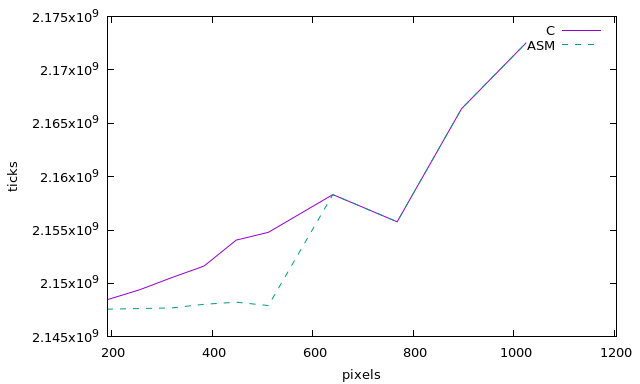
\includegraphics[scale=0.77]{imagenes/smalltiles-CvsASM.png}
	\caption{Comparación de los tiempos de ejecución de cada implementación}
	\label{smalltiles_asmvsc}
  \end{center}
\end{figure}

En la figura 1, se muestra las cantidad de ticks que se necesitaron para ejecutar el filtro en C y ASM.   Se hicieron mediciones para imagenes de distintos tamaños. Se puede observar que imagenes de 200 a 600 pixeles, el filtro en ASM se necesitaron menos ticks de reloj que en su version en C.
Las mediciones se realizaron según lo descrito al principio del informe en Ubuntu 16.04, con 4GB de memoria RAM DDR3 y un procesador Intel Core i3-3240 corriendo a una frecuencia de 3.4GHz.

\subsubsection{Experimentacion}
\textbf{Hipótesis}
\newline
La version ASM de este filtro depende que instrucciones usamos para organizar los pixeles que necesitamos tomar  y que necesitan estar en las replicas. En cada iteracion se utiliza la instrucción pshufdq para reorganizar los pixeles en xmm1 para su insercion en la imagen destino, pero la idea es probar si en vez de esa instrucción se puede utilizar instruciones de extract e insert para lograr el mismo y si es posible un mejor resultado.

\textbf{Resultados}
\\
Se realizaron medicion de ticks de reloj para imagenes de distintos tamaños. Lo que se hace en este experimento remplazar una instruccion por 3, para si se presenta una mejora en la implementacion. 
Las mediciones se realizaron según lo descrito al principio del informe en Ubuntu 14.04, con 4GB de memoria RAM DDR3 y un procesador Intel Core i3-3240 corriendo a una frecuencia de 3.4GHz.


\begin{figure}[H]
  \begin{center}
	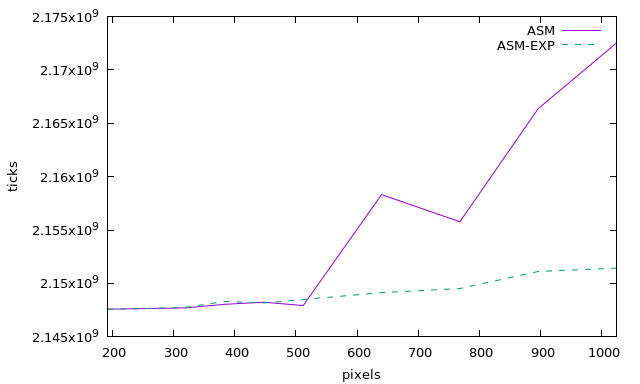
\includegraphics[scale=0.77]{imagenes/smalltiles-Exp.png}
	\caption{Comparación de los tiempos de ejecución}
	\label{rotar_exp}
  \end{center}
\end{figure}

En la figura 2 se puede notar que reemplazar esa instrucción presento una mejora en el rendimiento del filtro. Para las imágenes de 200 a 500 pixeles los cantidad de  ticks de ambos filtros son bastante similares presentado muy poca diferencia. A partir de imagenes de 500 o mas pixeles se nota que la cantidad de ticks del filtro experimento necesita es menor a la cantidad que el filtro original necesita, convirtiendo al filtro de experimento en mas eficiente que el original.

\newpage
\subsection{Rotar}
\subsubsection{Implementación}
Este filtro lo que hace es simplemente rotar los valores de los colores en los pixeles. Lo implementamos en muy pocas líneas en lenguaje ensamblador gracias a que utilizamos la instrucción \textit{shuffle} junto a una máscara (escrita como constante en memoria) que indica la nueva posición de cada valor en el píxel de la imagen destino. Por lo tanto, lo único que se realiza en cada iteración es la carga de la imagen de memoria en un registro, ejecutar la instrucción \textit{shuffle} y almacenar el registro en la posición de memoria del puntero a la imagen destino. 
\\Como los valores en los pixeles no son alterados de ninguna forma, no hay pérdida de precisión alguna.\\

Se itera sobre la imagen columna por columna, y, una vez que se terminó de recorrer una fila, se decrementa el contador que contiene la cantidad de filas a recorrer. De esta manera, una vez que dicho contador llegó a cero, se terminó de recorrer la imagen. Como se opera de a 4 pixeles por vez, se divide la cantidad de columnas (que están en pixeles) por cuatro y los punteros avanzan de a 16 bytes. No se puede operar de a más pixeles por vez porque cada uno ocupa 32 bits, entonces solo se pueden almacenar cuatro de ellos por vez en los registros de SIMD.\\


La implementación realizada en C itera sobre la imagen con dos ciclos anidados (avanzando por columnas), de a un píxel por vez. Simplemente rota los valores de los pixeles en la imagen destino. Si bien las operaciones se realizan de manera muy similar a la implementación en lenguaje ensamblador, esta última recorre la imagen más rápido al procesar de a 4 pixeles por iteración, por lo que el rendimiento debería ser mayor.\\

\begin{figure}[H]
  \begin{center}
	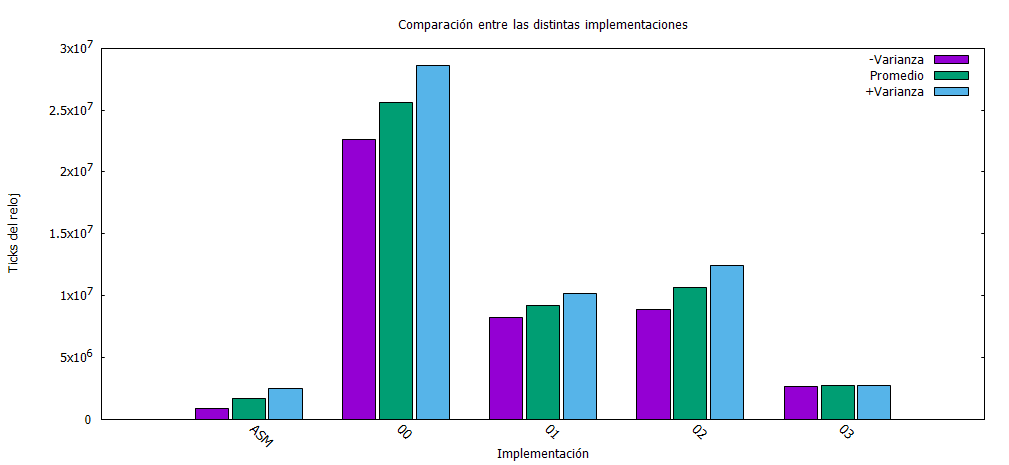
\includegraphics[scale=0.77]{imagenes/rotarC.png}
	\caption{Comparación de los tiempos de ejecución de cada implementación}
	\label{rotar_asmvsc}
  \end{center}
\end{figure}

Como se puede observar en~\ref{rotar_asmvsc}, la cantidad de \textit{ticks} de reloj necesarios para ejecutar el mismo filtro en su implementación en C es considerablemente mayor a aquellos necesarios para ejecutar el filtro en su implementación en lenguaje ensamblador, como era de esperarse. La diferencia aumenta a medida que aumenta el tamaño de la imagen, donde se puede observar que la versión en C tiene una complejidad lineal, mientras que la implementación en lenguaje ensamblador lo hace en un orden menor.\\
Las mediciones se realizaron según lo descrito al principio del informe en Ubuntu 14.04, con 4GB de memoria RAM DDR2 y un procesador Intel Core 2 Quad Q9550 corriendo a una frecuencia de 2830MHz.

\subsubsection{Experimentación}
\textbf{Hipótesis}
\newline
La instrucción principal de este filtro, como mencionamos anteriormente, es \textit{shuffle}. En esta experimentación queremos probar lo que ocurre si hacemos la rotación de valores de manera manual, simplemente desempaquetando y empaquetando los valores en las nuevas posiciones. Esto implica escribir más instrucciones y realizar un código más ilegible.
\\Como la cantidad de instrucciones ha aumentado considerablemente, creemos que el tiempo de ejecución será mayor, a pesar de que sean (probablemente) menos costosas que la operación \textit{shuffle}. Aun así, debería ser menor a la implementación en C. 
\newline

\textbf{Resultados}
\\Se realizó una medición de la cantidad de \textit{ticks} de reloj del CPU que conllevó ejecutar el filtro para los distintos tamaños de entrada. Únicamente se varió el tamaño de las imágenes y no sus componentes porque las cuentas a realizar son independientes de los valores cromáticos de la imagen, por lo que se descartó que puedan haber variaciones apreciables dependiendo de la imagen en sí.
\\Las mediciones se realizaron según lo descrito al principio del informe en Ubuntu 14.04, con 4GB de memoria RAM DDR2 y un procesador Intel Core 2 Quad Q9550 corriendo a una frecuencia de 2830MHz.\\

\begin{figure}[H]
  \begin{center}
	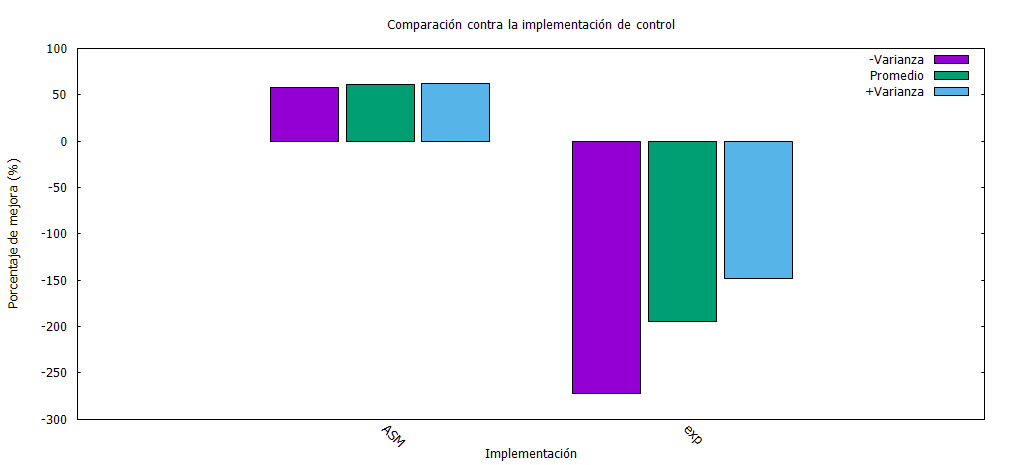
\includegraphics[scale=0.77]{imagenes/rotarExp.png}
	\caption{Comparación de los tiempos de ejecución}
	\label{rotar_exp}
  \end{center}
\end{figure}

Los resultados coinciden con lo esperado, donde los tiempos de ejecución del filtro operando con la instrucción \textit{shuffle} son menores al resto, y a su vez, la versión en C sigue siendo la menos eficiente, ya que opera píxel por píxel e implica más accesos a memoria. También podemos notar que las diferencias entre las implementaciones se hacen más notorias a medida que aumenta la cantidad de datos a procesar. Concluimos que el empaquetado y desempaquetado de datos conlleva un costo mayor para reordenar datos a su equivalente utilizando la instrucción \textit{shuffle}.

\newpage

\subsection{Pixelar}
\subsubsection{Implementación}
Como el filtro necesita la información de dos filas para realizar el promedio, recorremos tanto la imagen fuente como la imagen destino con dos punteros. Estos se mueven de forma paralela, es decir, en las mismas columnas pero en filas consecutivas. Al trabajar de esta forma y utilizando instrucciones SIMD podemos aplicar los cambios a ocho pixeles a la vez (cuatro por punteros).
\\Para no perder precisión, todas las operaciones necesarias para obtener los promedios se realizan en enteros. Una vez calculados (uno por grupo de 4 pixeles), se reemplazan los valores originales de los pixeles en la imagen destino por el valor promedio correspondiente.
\\Se itera sobre la imagen columna por columna, y, una vez que se terminaron de recorrer las dos filas paralelas, se decrementa el contador que contiene la mitad de la cantidad total de filas a recorrer. De esta manera, una vez que dicho contador llegó a cero, se terminó de recorrer la imagen. Como se opera de a 4 pixeles por puntero, se divide la cantidad de columnas (que están en pixeles) por cuatro y los punteros avanzan de a 16 bytes. A su vez, cuando se terminan de recorrer las filas, los punteros avanzan la cantidad de columnas multiplicado por cuatro (bytes), saltándose cada puntero una fila. No se puede operar de a más pixeles por vez porque cada uno ocupa 32 bits, por lo que solo se pueden almacenar cuatro de ellos a la vez en los registros de SIMD.
\\
\\
La implementación realizada en C itera sobre la imagen con dos ciclos anidados (avanzando por columnas) de a 4 pixeles por vez, avanzando de a dos columnas y dos filas a la vez. Simplemente se calcula el promedio en cuatro pixeles y se coloca este valor en la imagen destino en las posiciones de los pixeles procesados. Si bien las cuentas se realizan de manera muy similar a la implementación en lenguaje ensamblador, esta última recorre la imagen más rápido al procesar de a 8 pixeles por iteración, por lo que el rendimiento debería ser mayor.
\\
\begin{figure}[H]
  \begin{center}
	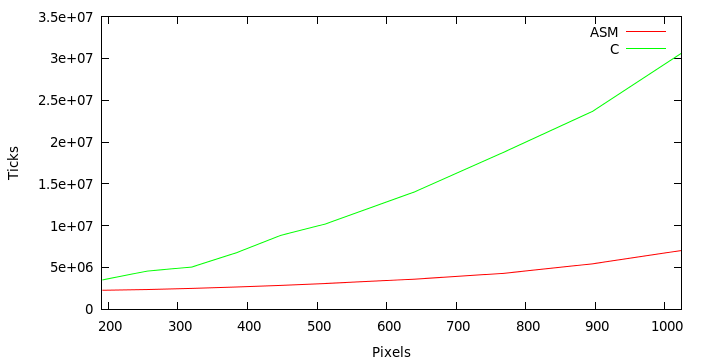
\includegraphics[scale=0.77]{imagenes/pixelarC.png}
	\caption{Comparación de los tiempos de ejecución de cada implementación}
	\label{pixelar_asmvsc}
  \end{center}
\end{figure}

Como se puede observar en~\ref{pixelar_asmvsc}, la cantidad de \textit{ticks} de reloj necesarios para ejecutar el mismo filtro en su implementación en C es considerablemente mayor a aquellos necesarios para ejecutar el filtro en su implementación en lenguaje ensamblador, como se suponía. La diferencia aumenta a medida que aumenta el tamaño de los datos de entrada, donde se puede observar que la implementación en C tiene una complejidad lineal, mientras que la implementación en lenguaje ensamblador lo hace en un orden más bajo.
\\
Las mediciones se realizaron según lo descrito al principio del informe en Ubuntu 14.04, con 4GB de memoria RAM DDR2 y un procesador Intel Core 2 Quad Q9550 corriendo a una frecuencia de 2830MHz.

\subsubsection{Experimentación}
\textbf{Hipótesis}
\newline
Dentro de las series de operaciones que ejecuta el filtro, existe una división entera que efectuamos con la instrucción \textit{psrld}. En esta experimentación queremos ver la diferencia, tanto en tiempo como en precisión, al utilizar una división de punto flotante. Entendemos que en este caso no tiene sentido utilizarla, porque los decimales que perdemos al utilizar la división entera los ibamos a descartar de todas formas, ya que la información en los pixeles se encuentra en enteros. Aún así, nos interesa ver las diferencias entre ambos métodos. Suponemos que la diferencia en rendimiento no debería variar mucho, ya que la división en punto flotante se realiza a través de una tabla \textit{hardcodeada}, y analizaremos la variación en la precisión (la cual debería ser mayor para la división en punto flotante).
\newline
\\
\textbf{Resultados}
\\Se realizó una medición de la cantidad de \textit{ticks} de reloj del CPU que conllevó ejecutar el filtro para los distintos tamaños de entrada. Únicamente se varió el tamaño de las imágenes y no sus componentes porque las cuentas a realizar son independientes de los valores cromáticos de la imagen, por lo que se descartó que puedan haber variaciones apreciables dependiendo de la imagen en sí.
\\Las mediciones se realizaron según lo descrito al principio del informe en Ubuntu 14.04, con 4GB de memoria RAM DDR2 y un procesador Intel Core 2 Quad Q9550 corriendo a una frecuencia de 2830MHz.
\\

\begin{figure}[H]
  \begin{center}
	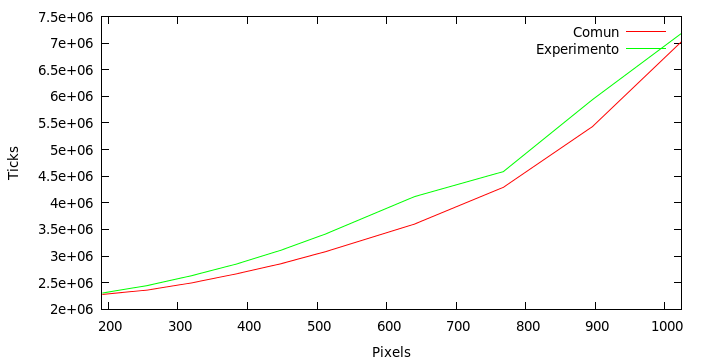
\includegraphics[scale=0.77]{imagenes/pixelarExp.png}
	\caption{Comparación de los tiempos de ejecución}
	\label{pixelar_exp}
  \end{center}
\end{figure}

Los resultados indican que, si bien existe una tabla \textit{hardcodeada} para las operaciones costosas como multiplicación y división en punto flotante, su costo sigue siendo mayor a aquél de operar la división \textit{shifteando}, pero la diferencia no es tan notable como entre la implementación en C y en lenguaje ensamblador, denotada en la figura~\ref{pixelar_asmvsc}. Es decir, efectivamente el costo insumido no es tan grande, a pesar de que involucre operar con \textit{floats}.
\\Una vez determinado que insume un mayor costo la operación con punto flotante, falta analizar la diferencia en la precisión.
\\Para analizar qué tanta diferencia hay entre un resultado y otro, utilizamos la herramienta \textit{bmpdiff}, generando imágenes que muestran la diferencia píxel a píxel para cada componente. El parámetro epsilon de la herramienta \textit{bmpdiff} se fijó en cero.
\\

\begin{figure}[H]
  \begin{center}
	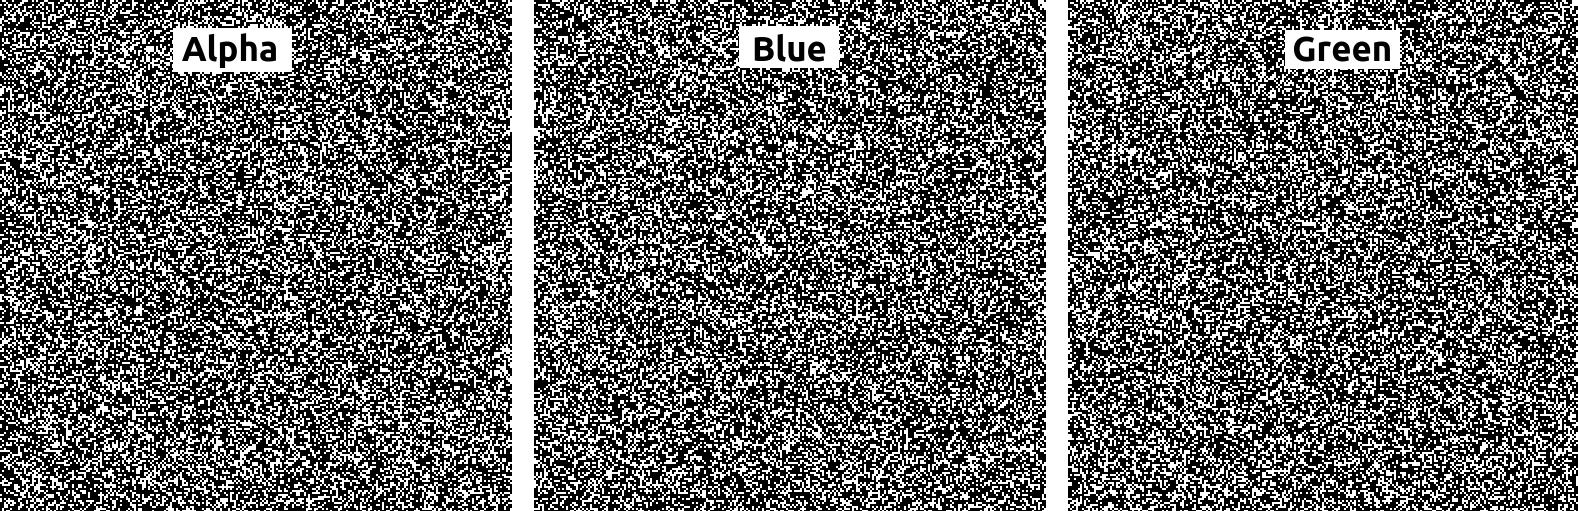
\includegraphics[scale=0.40]{imagenes/pixelardiffExp.jpeg}
	\caption{Diferencia píxel a píxel para cada componente}
	\label{pixelar_diff}
  \end{center}
\end{figure}

Como se puede observar, las diferencias en la imagen son uniformes, lo que confirma que el color no tuvo incidencia en las operaciones. Si bien parecen ser muchos los pixeles con distintos valores, la diferencia es prácticamente nula: al ejecutar \textit{bmpdiff} una vez más pero con el parámetro epsilon en 1 (es decir, permitiendo que haya un margen de error de $+/-$ uno para cada color) se obtuvieron imágenes en negro para todas las componentes. En otras palabras, la diferencia de precisión es mínima, ya que solo difieren en uno cada componente de cada píxel. Sabiendo esto podemos concluir que en algunos casos puede ser preferible acarrear un mayor costo operando con punto flotante, en caso de requerir la mayor precisión posible.

\newpage
\subsection{Combinar}
\subsubsection{Implementación}
Ya que el filtro se ejecuta sobre el reflejo vertical de la imagen fuente, en lenguaje ensamblador se mantiene como invariante un puntero a la imagen invertida. Es decir, a medida que se recorre la matriz de la imagen fuente, este puntero la recorre de atrás hacia delante. Por lo tanto, avanza restándole posiciones de memoria. Por otro lado, como recorre de atrás hacia delante, levanta los pixeles de memoria de manera invertida, por lo que en cada iteración del ciclo, luego de levantar los pixeles, se reordenan de manera que coincidan vectorialmente con aquellos contenidos en el registro que opera sobre la matriz comúnmente (es decir, de delante hacia atrás).

Para no perder precisión, antes de realizar la resta entre pixeles, se extiende cada componente del píxel a un entero de 32 bits y se hacen todas las operaciones intermedias operando como \textit{floats}. Además, como la cuenta incluye el uso de constantes, las mismas se guardan en memoria como datos de solo lectura. Para no perder rendimiento levantándolas en cada iteración del ciclo, se guardan en un registro específico antes de empezar a recorrer la imagen.

Se itera sobre la imagen columna por columna, y, una vez que se terminó de recorrer una fila, se decrementa el contador que contiene la cantidad de filas a recorrer. De esta manera, una vez que dicho contador llegó a cero, se terminó de recorrer la imagen. Como se opera de a 4 pixeles por vez, se divide la cantidad de columnas (que están en pixeles) por cuatro y los punteros avanzan de a 16 bytes. No se puede operar de a más pixeles por vez porque cada uno ocupa 32 bits, entonces solo se pueden almacenar cuatro de ellos por vez en los registros de SIMD.
\bigskip

La implementación realizada en C itera sobre la imagen con dos ciclos anidados (avanzando por columnas), de a un píxel por vez. Las operaciones se realizan con una variable auxiliar de tipo \textit{float} y luego se castea la misma al tipo de dato de la estructura correspondiente al color del píxel (\textit{unsigned char}). Si bien las cuentas se realizan de manera muy similar a la implementación en lenguaje ensamblador, esta última recorre la imagen más rápido al procesar de a 4 pixeles por iteración, por lo que el rendimiento debería ser mayor. 
\\
\begin{figure}[H]
  \begin{center}
	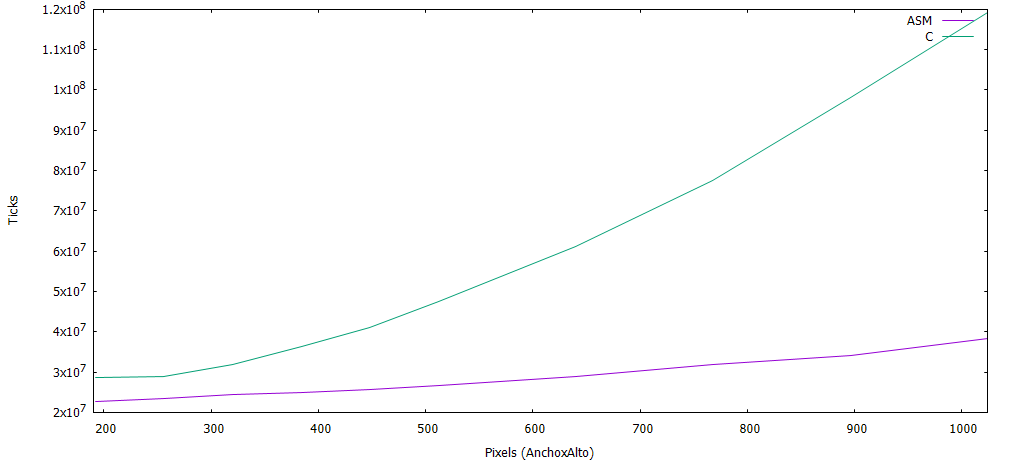
\includegraphics[scale=0.66]{imagenes/combinarC.png}
	\caption{Comparación de los tiempos de ejecución de cada implementación}
	\label{combinar_asmvsc}
  \end{center}
\end{figure}

Como se puede observar en~\ref{combinar_asmvsc}, la cantidad de \textit{ticks} de reloj necesarios para ejecutar el mismo filtro en su implementación en C es considerablemente mayor a aquellos necesarios para ejecutar el filtro en su implementación en lenguaje ensamblador, como era de esperarse. La diferencia aumenta a medida que aumenta el tamaño de la imagen, donde se puede observar que la implementación en C tiene una complejidad lineal, mientras que la implementación en lenguaje ensamblador lo hace en un orden más bajo.

Las mediciones se realizaron según lo descrito al principio del informe, con un parámetro \textit{alpha} de 128, en Ubuntu 16.04, con 1GB de memoria RAM DDR3 y un procesador Intel Core i3-2100 corriendo a una frecuencia de 3096MHz.
\subsubsection{Experimentación}
\textbf{Hipótesis}
\newline

Ya que el filtro consta de ejecutar una serie de operaciones, la mayor complejidad del mismo se encuentra en las cuentas que hay que realizar. Si bien la suma y resta de enteros no insume prácticamente ningún costo, dentro de las operaciones a realizar se encuentra una multiplicación con valores de punto flotante (\textit{alpha}) y la división por 255.0. Ya que \textit{alpha} representa un valor comprendido en [0.00;255.0], si se lo interpreta como un entero, el truncamiento no representa una pérdida de precisión muy importante, y el rendimiento obtenido debería compensar tal pérdida. Así mismo, se puede realizar algo similar con la división por 255.0. Si bien la división por enteros es costosa, es posible dividir el resultado parcial obtenido por 256 en lugar de 255. La operación no insume un mayor costo porque simplemente consta de \textit{shiftear} los bits, en lugar de realizar una división propiamente dicha. Además, ya que la operación se realizaría únicamente con enteros, no es necesario hacer \textit{casteos} intermedios entre punto flotante y enteros, los cuales son muy costosos.
\newline
\\
\textbf{Resultados}

Se realizó una medición de la cantidad de \textit{ticks} de reloj del CPU que conllevó ejecutar el filtro para los distintos tamaños de entrada. Únicamente se varió el tamaño de las imágenes y no sus componentes porque las cuentas a realizar son independientes de los valores cromáticos de la imagen, por lo que se descartó que puedan haber variaciones apreciables dependiendo de la imagen en sí. Por otro lado, el parámetro \textit{alpha} se fijó en 128.

Las mediciones se realizaron según lo descrito al principio del informe, en Ubuntu 16.04, con 1GB de memoria RAM DDR3 y un procesador Intel Core i3-2100 corriendo a una frecuencia de 3096MHz.
\\
\begin{figure}[H]
  \begin{center}
	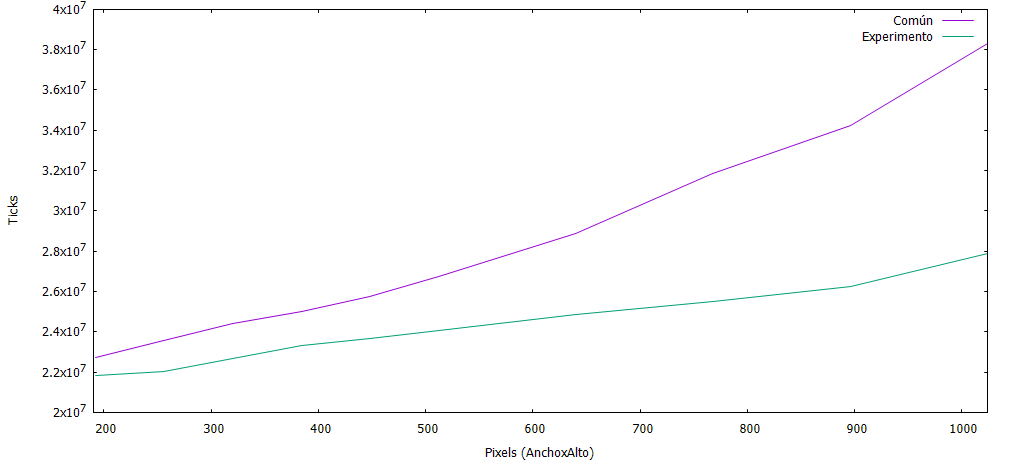
\includegraphics[scale=0.66]{imagenes/combinarExp.png}
	\caption{Comparación de los tiempos de ejecución}
	\label{combinar_exp}
  \end{center}
\end{figure}

Los resultados condicen con lo esperado, donde los tiempos de ejecución del filtro operando únicamente con enteros son menores a aquellos utilizados para operar sin pérdida de precisión. La diferencia se hace más notable a medida que aumenta el tamaño de la imagen, pero no es tan notable como la diferencia entre la implementación en C y en lenguaje ensamblador, denotada en la figura~\ref{combinar_asmvsc}.

Sin embargo, obteniendo la diferencia porcentual entre los distintos tiempos de ejecución, se obtiene que para datos de entrada chicos, la mejora ronda entre el 4 y el 8\%, mientras que para los tamaños de imagen más grande, la diferencia entre operar con enteros y operar con números en punto flotante de precisión simple llega al 40\%. Queda claro que el rendimiento mejora al operar con enteros, pero falta analizar cuánta precisión se pierde.
\bigskip

Para analizar qué tanta diferencia hay entre un resultado y otro, utilizamos la herramienta \textit{bmpdiff}, generando imágenes que muestran la diferencia píxel a píxel para cada componente. Las imágenes se obtuvieron corriendo el filtro con el parámetro \textit{alpha} de valor 127.484, para realzar las diferencias por pérdida de precisión. El parámetro epsilon de la herramienta \textit{bmpdiff} se fijó en cero.
\\
\begin{figure}[H]
  \begin{center}
	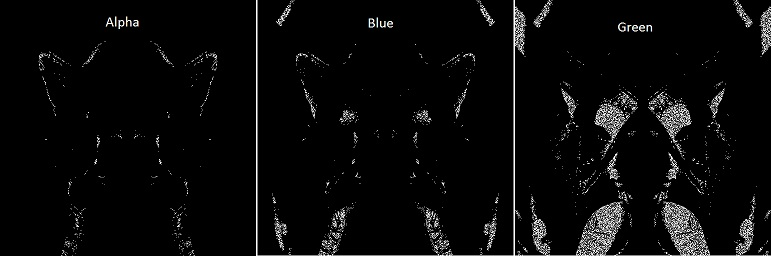
\includegraphics[scale=0.66]{imagenes/diffExp.jpg}
	\caption{Diferencia píxel a píxel para cada componente}
	\label{combinar_diff}
  \end{center}
\end{figure}

Como se puede observar, la mayor diferencia se obtiene en la componente verde, mientras que la roja (no incluida en la figura) no poseía diferencias. Si bien parecen ser varios los pixeles con distintos valores, la diferencia es prácticamente nula: al ejecutar \textit{bmpdiff} una vez más pero con el parámetro epsilon en 1 (es decir, permitiendo que haya un margen de error de $+/-$ uno para cada color) se obtuvo imágenes en negro para todas las componentes. En otras palabras, la pérdida de precisión es mínima, ya que solo difieren en uno cada componente de cada píxel, mientras que la mejora en rendimiento es notable, especialmente para imágenes de mayor tamaño. Por lo tanto, se concluye que es preferible utilizar la implementación con enteros si la precisión no es muy importante, especialmente teniendo en cuenta la mejora en tiempos de ejecución para imágenes grandes.

\newpage

\subsection{Colorizar}
\subsubsection{Implementación}

El filtro Colorizar trabaja con los valores máximos de los colores de aquellos pixeles que se encuentren alrededor del píxel a procesar, incluyéndolo. Por esta razón, se mantuvo un puntero a la fila anterior y posterior del píxel a procesar, de manera tal de poder aprovechar las instrucciones de SIMD para realizar varias comparaciones simultáneamente. Por otro lado, como las operaciones a realizar incluyen el uso de constantes, las mismas se cargaron en memoria (en la sección de datos de solo lectura) y luego a los registros al inicio del programa. Además, por enunciado, la primera y última fila, así como la primera y última columna, no se procesan. Por lo tanto, el puntero a la imagen destino comienza una fila y una columna más adelante. Lo mismo ocurre para el puntero de la imagen fuente que contiene los pixeles a procesar. 

Debido a que no se procesa la primera y última columna (siendo la cantidad total de columnas múltiplo de cuatro), y solo se pueden realizar comparaciones de a cuatro pixeles por vez, el algoritmo implementado en lenguaje ensamblador procesa de a dos pixeles por iteración.

Luego de obtener los valores máximos de cada color de los pixeles a procesar y sus vecinos, se comparan entre ellos generando máscaras. Estas mismas máscaras aprovechan el valor \textit{true} de las comparaciones interpretándolas como un $-1$ y, luego de obtener su complemento, agregando el valor $1$ donde haya ceros. De esta manera, al multiplicar por el registro que contiene al parámetro $\alpha$, se obtiene $-\alpha$ en aquellos lugares donde la comparación haya resultado falsa y $\alpha$ en aquellos lugares donde la comparación haya resultado verdadera. Luego solo resta sumar por la constante $1.0$ cargada previamente en un registro. 

Para obtener los mínimos entre los resultados obtenidos y el valor $255$, se realiza una operatoria muy similar utilizando máscaras junto con la operación lógica AND y luego sumando. El valor $alpha$ original de los pixeles es copiado al resultado una vez realizadas las operaciones.
\bigskip

En el caso de la implementación realizada en C, la iteración sobre la matriz opera de manera muy similar, salteando la primera y última fila y la primera y última columna de cada fila, con la diferencia de que se procesa de a un píxel por vez. Además, para buscar el máximo, se realiza otro bucle iterando sobre los vecinos del píxel, por lo que se espera que la diferencia de rendimiento entre una implementación y otra sea considerable (ya que realiza bastantes más accesos a memoria que la implementación en lenguaje ensamblador).

Solo se varió el tamaño de las imágenes a probar porque, si bien los máximos dependen del valor de los colores, las comparaciones se efectúan independientemente de sus valores, y la operación a realizar (suma o resta) según los resultados de las mismas es equivalente en términos de rendimiento.
\\
\begin{figure}[H]
  \begin{center}
	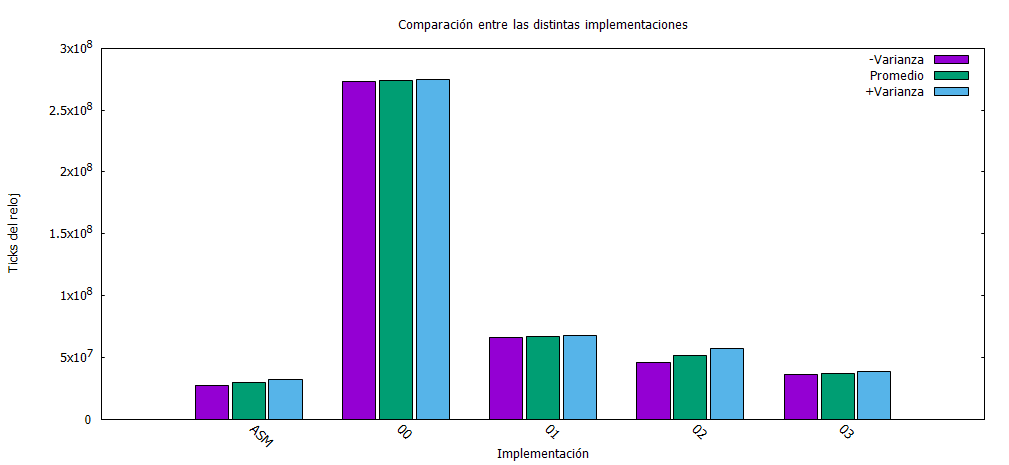
\includegraphics[scale=0.66]{imagenes/colorizarC.png}
	\caption{Comparación entre las distintas implementaciones}
	\label{colorizar_asmvsc}
  \end{center}
\end{figure}

Como se puede observar en la figura~\ref{colorizar_asmvsc}, la diferencia entre la implementación en lenguaje ensamblador y aquella en C es muy considerable, donde la implementación en C consume muchos más \textit{ticks} de reloj a medida que aumenta el tamaño de los datos de entrada y su contraparte lo hace en un orden bastante menor. Suponemos que la diferencia es más notable que en otros filtros (teniendo en cuenta que se procesa únicamente de a dos pixeles por iteración en lugar de a cuatro, como los demás) por la cantidad de accesos a memoria que requiere la implementación en C para buscar el máximo.
\\
\subsubsection{Experimentación}
\textbf{Hipótesis}

Dado que el filtro se caracteriza por buscar los máximos en un cuadrado alrededor del píxel a procesar, muchos resultados se solapan. Es decir, los máximos de cada columna se calculan más de una vez. Si bien esto no representa un problema para la implementación en lenguaje ensamblador (ya que las comparaciones se realizan de manera vectorial y los accesos a memoria no se reducen), para la implementación en C se puede reducir considerablemente los accesos a memoria si se reusan los resultados, manteniendo los resultados parciales (como una suerte de programación dinámica). De esta manera, excepto para la primera iteración de cada fila, ya se consiguieron los máximos de dos de las tres columnas a evaluar.

Almacenando estos resultados parciales, se reducen los accesos a memoria en un orden no menor, dado que solo es necesario calcular el máximo de la columna siguiente al píxel a procesar. En total, la cantidad de accesos a memoria deberían reducirse en $2/3$ (aproximadamente, ya que para la primera iteración de cada fila sigue siendo necesario calcular los máximos de las tres columnas).

Los accesos a memoria deberían conformar una parte considerable del costo insumido por la implementación en C, por lo que se espera que, al reducirlos, la diferencia de tiempos entre la implementación en ensamblador y la implementación en C sea menor a aquella de los demás filtros (dado que en este filtro se procesa de a dos en lugar de a cuatro).
\\
\textbf{Resultados}

Para analizar lo dicho, se ejecutó ambas implementaciones en C de la manera descrita al principio del trabajo práctico y se comparó ambos resultados.
\\
\begin{figure}[H]
  \begin{center}
	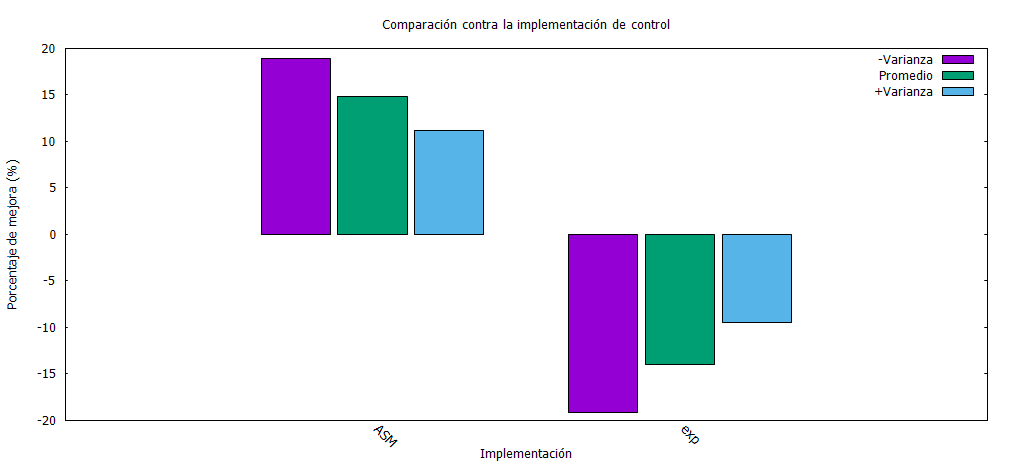
\includegraphics[scale=0.66]{imagenes/colorizarExp.png}
	\caption{Comparación entre las distintas implementaciones en C}
	\label{colorizar_exp}
  \end{center}
\end{figure}

Como se puede observar en la figura~\ref{colorizar_exp}, efectivamente se redujo el tiempo de ejecución, acentuándose la diferencia para imágenes de mayor tamaño. Calculando la diferencia porcentual entre ambas implementaciones, para imágenes de menor tamaño se obtuvo una mejora promedio del 15\% y para datos de entrada considerablemente más grandes, se mejoró en un 45\% aproximadamente.
Comparando el rendimiento con la implementación en lenguaje ensamblador, se obtuvo lo siguiente:
\\
\begin{figure}[H]
  \begin{center}
	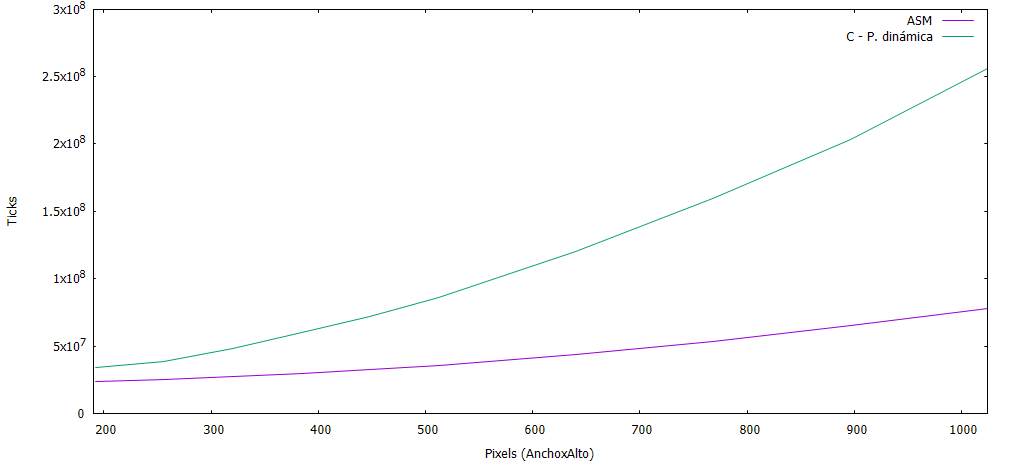
\includegraphics[scale=0.66]{imagenes/colorizarExpASM.png}
	\caption{Comparación entre las distintas implementaciones}
	\label{colorizar_expASM}
  \end{center}
\end{figure}

En esta figura es fácilmente observable que la diferencia entre la implementación en lenguaje ensamblador y su análoga en C es mucho menor a comparación de los resultados obtenidos en la figura~\ref{colorizar_asmvsc}. Estos resultados condicen con lo planteado anteriormente, además de denotar una diferencia entre implementaciones menor a comparación de los demás filtros, ya que estos procesan de a cuatro pixeles mientras que este solo lo hace de a dos, comprobando lo dicho en la hipótesis. 

\end{document}
